%% LyX 2.1.4 created this file.  For more info, see http://www.lyx.org/.
%% Do not edit unless you really know what you are doing.
\documentclass[12pt,british,sort&compress]{article}
\usepackage{mathptmx}
\renewcommand{\familydefault}{\rmdefault}
\usepackage[T1]{fontenc}
\usepackage[latin9]{inputenc}
\usepackage{geometry}
\geometry{verbose,tmargin=2cm,bmargin=2cm,lmargin=2cm,rmargin=2cm,headheight=2cm,headsep=2cm,footskip=1.5cm}
\usepackage{refstyle}
\usepackage{float}
\usepackage{rotfloat}
\usepackage{amssymb}
\usepackage{graphicx}
\usepackage{esint}

\makeatletter

%%%%%%%%%%%%%%%%%%%%%%%%%%%%%% LyX specific LaTeX commands.

\AtBeginDocument{\providecommand\figref[1]{\ref{fig:#1}}}
%% Because html converters don't know tabularnewline
\providecommand{\tabularnewline}{\\}
\RS@ifundefined{subref}
  {\def\RSsubtxt{section~}\newref{sub}{name = \RSsubtxt}}
  {}
\RS@ifundefined{thmref}
  {\def\RSthmtxt{theorem~}\newref{thm}{name = \RSthmtxt}}
  {}
\RS@ifundefined{lemref}
  {\def\RSlemtxt{lemma~}\newref{lem}{name = \RSlemtxt}}
  {}


\@ifundefined{date}{}{\date{}}
%%%%%%%%%%%%%%%%%%%%%%%%%%%%%% User specified LaTeX commands.

\usepackage{hyperref}
\usepackage{xcolor}
\hypersetup{
    colorlinks,
    linkcolor={red!50!black},
    citecolor={blue!50!black},
    urlcolor={blue!80!black}
}


%removes unecessary spaces from bullet listing
\usepackage{enumitem}
\setlist{nolistsep}

%for fitting more citations
\usepackage{multicol}


\bibliographystyle{unsrt}
%to make separate references
%\usepackage[sectionbib]{chapterbib}
%\usepackage[english]{babel}
%\usepackage{biblatex}
%\usepackage[style=authoryear,backend=biber,refsection=none]{biblatex}
%\bibliography{MIS2015.bib}
%\addbibresource{{/home/atul/SparkleShare/ULB repo/intermediate/furtherScholarship/tex/MIS2015.bib}}
%\addbibresource{{/home/atul/SparkleShare/ULB repo/intermediate/furtherScholarship/tex/MIS2015}}
%\addbibresource{{MIS2015}}
%\addbibresource{{MIS2015.bib}}

\makeatother

\usepackage{babel}
\begin{document}
\begin{flushright}
\pagenumbering{roman}\large{FRIA CALL 2016 - FRIA-B1}
\par\end{flushright}

\hfill{}%
\begin{tabular}{|l|l|}
\hline 
\multicolumn{1}{|l|}{Full name of the applicant} & \multicolumn{1}{l|}{Atul Singh Arora }\tabularnewline
\hline 
SEMAPHORE Application ID & 29379721\tabularnewline
\hline 
\end{tabular}\hfill{}

\medskip{}


\begin{center}
\huge{SCIENTIFIC SECTION OF THE PROPOSAL}
\par\end{center}

\begin{center}
Main language chosen = English
\par\end{center}

\clearpage{}

\pagenumbering{arabic}


\section{DESCRIPTION OF THE RESEARCH PROJECT}

%\begin{refsection}



\subsection{Goals of the Research}

Current information processing models are fundamentally limited in
terms of speed, efficiency, security and privacy, as they assume a
simplified representation of the world, relying on classical physics.
In the past few decades, research in the field of quantum information
processing has been carried out to break this barrier by exploiting
quantum phenomena. This has led to breakthrough results such as Bennett
and Brassard's informationaly secure quantum key distribution protocol~\cite{BB84}
and Shor's efficient factoring algorithm~\cite{shor94} which suggest
that future large-scale network of computing devices will be able
to communicate both efficiently and securely using quantum resources.

Despite steady progress, including practical implementations of quantum
key distribution schemes, there are both technological limitations
and theoretical barriers. The development of algorithms and protocols
exploiting such a quantum network to its full capacity is also hindered
by the inherent difficulty at characterizing interactive quantum communication
models. As a consequence, only limited techniques are known for studying
quantum communication complexity, and the development of fundamental
cryptographic primitives such as quantum coin flipping requires complicated
tools that make it extremely hard to derive explicit protocols.

The overall aim of this research project is to take a fresh start
towards quantum communication protocols by approaching their theoretical
foundations from a new perspective. More precisely, our objectives
are the following: 
\begin{itemize}
\item The development of a new framework to study quantum communication
protocols based on continuous~time Hamiltonian evolution. 
\item New techniques to obtain strong lower bounds in quantum communication
complexity and matching efficient protocols. 
\item Practical and optimal quantum protocols for cryptographic primitives,
in particular for coin flipping.
\end{itemize}

\subsection{State of the Art}

Communication complexity is a computational model first introduced
by Yao~\cite{Yao79} where two distant players, Alice and Bob, each
receive an input, $x$ and $y$, respectively, and their goal is to
compute a function $f(x,y)$. To this end, they must communicate,
and the communication complexity is defined as the minimum number
of bits exchanged by Alice and Bob in order to compute the function
with error at most $\epsilon$. In addition to being a quite natural
computational model on its own, communication complexity also found
many applications, not only for proving bounds via reductions for
other computational models (decision trees, streaming algorithms),
but also for more practical problems such as the design of VLSI circuits
(see also {[}KN97->add to bibtex file{]}). 

For this reason, communication complexity has been extensively studied
but progress has been quite slow due to the difficulty at developing
good lower and upper bound techniques. In particular, the famous log-rank
conjecture {[}LS88->add to bibtex file{]}, which states that the communication
complexity of a function is bounded from above by a constant power
of the rank of its communication matrix $M_{x,y}=f(x,y)$ remains
open despite decades of attempts to prove it. 

Over the last few years, a new approach to communication complexity
problems based on information theory {[}define this? Not sure it is
necessary{]} has attracted a lot of interest. This approach can not
only be used to prove lower bounds on the usual model, but also leads
to a new model called information complexity, where the cost of a
communication protocol no longer corresponds to the length of the
communicated messages, but rather to their information content (see
e.g.~\cite{Bra12}). Information complexity is also equivalent to
amortized communication complexity {[}BW12->add to bibtex file{]},
and therefore leads to an interactive analogue of Shannon compression
{[}define shannon compression first maybe? I think it is fine{]}.
It has recently been shown that some lower bound techniques for communication
complexity also lower bound information complexity~\cite{KLL+14}.
These techniques draw an interesting connection with the notion of
Bell inequalities studied in the context of quantum nonlocality, which
makes it possible to define natural extensions of these lower bound
techniques to quantum communication complexity~\cite{LLR12}, an
extension of communication complexity where the players can exchange
quantum messages. This line of research is quite promising as the
set of lower bound techniques for quantum communication complexity
is currently even more limited than for its classical counterpart. 

Note that closely related computational models are much better understood,
such as quantum query complexity {[}define it? WE could say that this
is the quantum analogue of query complexity or \textquotedblleft decision
tree complexity\textquotedblright , but we don\textquoteright t have
enough space to define it in more details{]}, which in the bounded-error
case is now known to be characterized by a semidefinite program called
the adversary bound~\cite{LMRSS11}. The proof of this fundamental
result is facilitated by considering a generalization of the model
where the goal is not to compute a function but rather to generate
a quantum state~\cite{AMRR11}. More recently, an alternative proof
of this was provided by my promoter by considering a continuous-time
model of quantum query complexity~\cite{BR14}. 

Coin flipping is a fundamental cryptographic primitive where two distrustful
parties need to remotely generate a shared unbiased random bit. A
cheating player can try to bias the output bit towards a preferred
value. For weak coin flipping, each player has a given preferred value:
for example, Alice wants to bias towards 0 while Bob wants to bias
towards 1. A weak coin-flipping protocol has bias $\epsilon$ if neither
Alice nor Bob can force the outcome towards her/his preferred value
with probability more than $1/2+\epsilon$. For strong coin flipping,
there is no a priori preferred values, and the protocol has bias $\epsilon$
if neither Alice nor Bob can force the outcome towards any value with
probability more than $1/2+\epsilon$. Under information-theoretic
security, neither weak nor strong coin flipping is possible with non-trivial
bias in the classical setting: there always exists a player that can
force any outcome with probability 1. However, the situation is quite
different in the quantum world. Indeed, strong coin-flipping protocols
with bias strictly less than $1/2$ have been shown, the best known
explicit protocol having bias $1/4$~\cite{Ambainis04b}. Nevertheless,
Kitaev showed a lower bound of $1/\sqrt{2}-1/2$ for the bias of any
quantum strong coin flipping~\cite{Kitaev03}, so an arbitrary small
bias is not possible. 

As for weak coin flipping, explicit protocols have been shown with
bias as low as $1/6$~\cite{Mochon05}. In a breakthrough result,
Mochon even proved in 2007 the existence of a quantum weak coin-flipping
protocol with bias $\epsilon$ for any $\epsilon>0$, hence showing
that near-perfect weak coin flipping is theoretically possible~\cite{Mochon07}.
This fundamental result for quantum cryptography unfortunately comes
with the important drawback that the proof of existence is non-constructive:
indeed, it is based on successive reductions from a protocol to different
versions of so-called point games, a formalism introduced by Kitaev
in order to study coin flipping. As a consequence, the structure of
the protocol whose existence is proved is unfortunately lost during
a long and technical sequence of reductions (the article is 80-page
long). Moreover, this article was never peer-reviewed, and it took
years before the proof was systematically verified by independent
researchers. While this verification also led to a simplified version
of the proof~\cite{ACG+14} (only 50-page long!), to this date, more
than 9 years after the original proof of existence, nobody has been
able to turn it into an explicit weak coin-flipping protocol. This
is not due to a lack of trying: experts have used various approaches
ranging from distilling a protocol from the theoretical proof of existence
to numerical search. For example, despite many optimization techniques,
the extensive numerical calculations in~\cite{NST14} did not return
a single protocol with a better bias than what was previously known.
While this last reference concerns strong coin-flipping protocols,
the problems are closely related, as it was shown that an explicit
quantum protocol for weak coin flipping would provide, via black-box
reductions, optimal protocols for strong coin flipping~\cite{CK09}
and oblivious transfer (another fundamental cryptographic primitive)
as well~\cite{CK11}. This makes the absence of explicit weak coin-flipping
protocols even more frustrating.


\subsection{Research Project}

\textbf{Continuous-time communication.} The main originality of my
research project is to consider a continuous-time model to study communication
complexity and cryptographic primitives. This is in sharp contrast
with the state of the art where virtually all interactive communication
models assume discrete-time protocols, where the communication travels
back and forth between the communicating players. The continuous-time
model I propose to study assumes that the players interact via a shared
``messaging'' system that can be coupled continuously in time to their
local workspace. More precisely, assume that Alice and Bob have private
quantum registers $A$ and $B$, and share a common message register
$M$. Alice can apply a Hamiltonian $H_{A}$ to her register and an
interaction Hamiltonian $H_{AM}$ to the combined system composed
of $A$ and $M$. Similarly Bob can apply $H_{B}$ and $H_{BM}$.
The complete Hamiltonian may be written as $H=H_{A}\otimes\mathbb{I}_{MB}+H_{AM}\otimes\mathbb{I}_{B}+\mathbb{I}_{A}\otimes H_{MB}+\mathbb{I}_{AM}\otimes H_{B}.$
Note that the traditional discrete-time communication model can be
seen as a special case of this model where at any point in time, either
$H_{AM}$ or $H_{BM}$ is zero. Conversely, any continuous-time protocol
may be approached by a discrete-time protocol via a Trotter expansion.
For this reason, the continuous-time model also provides a new approach
to study the usual discrete-time model. The first task of our PhD
project will be to formalize this general framework of continuous-time
communication and its connection the usual discrete-time model, before
we can use this framework in different contexts, namely communication
complexity and the design of cryptographic primitives. 

\textbf{Communication complexity.} We can define a continuous-time
model of communication complexity by considering the time required
to evolve the system to the desired state as a measure of complexity
(for this measure to be non-trivial, we need to impose energy constraints,
in that the norms of $H_{AM}$ and $H_{BM}$ must be bounded by some
constant $\le1$). An important task will be to prove tight bounds
between the usual (discrete-time) model and this new model, using
the general connection described above. From there, we propose to
develop new techniques to bound the continuous-time communication
complexity, which will in turn imply new bounds for the usual model.
Note that the most powerful known methods to prove bounds on communication
complexity require combinatorial techniques, due to the combinatorial
structure of interactive protocols where messages are sent back and
forth. It is quite likely that the algebraic structure of continuous-time
protocols might lead to a simpler analysis and therefore bound techniques
that are easier to apply (note that there also exist algebraic bound
techniques for the usual model of communication complexity, but while
they are typically easier to apply they are also less powerful and
therefore sometimes not sufficient). Another modification of the model
we propose to exploit is an extension to quantum state generation,
where instead of computing a function $f(x,y)$ (where $x$ and $y$
are Alice\textquoteright s and Bob\textquoteright s inputs), the goal
is to create a joint quantum state $\psi_{xy}$. This extension was
quite useful to simplify the study, up to the full characterization,
of quantum query complexity, and we hope to benefit from the same
advantage here. Indeed, even if the initial and final states of a
protocol are taken from a finite set of possibilities, as is the case
when computing a function, intermediate states of the protocol can
be arbitrary, and focusing on the singular properties of the states
at the beginning and the end of the protocol might obscure the general
dynamical properties. This is especially true for the continuous-time
model I propose to explore, since in that case the intermediate states
of the protocol follow a continuous path in the Hilbert space. In
order to design new techniques to prove lower bounds on this extended
model, I propose to combine these new ideas to recent techniques for
the usual discrete-time models, in particular techniques based on
information theory, as well as bounds derived from the notion of Bell
inequalities studied in the context of quantum non-locality {[}see
above, maybe add the same references here{]}. Finally, we also intend
to study continuous time models in the purview of classical communication
complexity where the Schr�dinger equation is replaced by appropriate
Euler Lagrange equations and is expected to yield a unified characterization
of communication complexity. We intend to study similar questions;
equivalence between continuous and discrete models and characterization
of complexity models using new bounding techniques. 

\textbf{Cryptography.} Constructing explicit optimal quantum protocols
for cryptographic primitives will be among the second main targets
of this project (see \figref{Expected-Research-Flow}). We will first
focus on weak coin flipping, not only because it can lead via reductions
to protocols for other primitives such as strong coin flipping and
bit commitment~\cite{CK09,CK11}, but also because my promoter has
already obtained some promising preliminary results. More precisely,
he has recently discovered that the best known quantum protocol for
weak coin flipping~\cite{Mochon05}, achieving bias $1/6$, can be
obtained by discretizing a continuous-time communication protocol
of the type we have defined above. This construction gives more insight
on how the protocol works and therefore provides a new approach to
extend it and break the limit of bias $1/6$, which resisted all researchers
for more than a decade. Indeed, while Mochon's original construction
requires taking the limit of an infinite number of discrete steps,
this new construction immediately yields a protocol as a continuous
evolution, which is easier to analyze and provides more intuition.
Our strategy will be to exploit this new intuition to finally break
the barrier corresponding to bias $1/6$. In order to do so, we propose
to adapt to this framework a technique introduced by Feynman in his
early works on quantum computers~\cite{Feynman86}, consisting in
constructing the history state of a computation, that is, $\left|\Psi\right\rangle =\sum_{t=0}^{T}\left|\psi_{t}\right\rangle \left|t\right\rangle $.
We believe that this might be the key to obtaining better biases,
because this states involves at the same ``physical time'' all states
of the protocol at different ``logical'' times, and therefore has
a structure which is very similar to the so-called ``time-independent
point games'' that Mochon used to prove (in a non-constructive manner)
the existence of protocols with arbitrarily low biases~\cite{Mochon07}.
In the case of a continuous-time protocol, the history state reads
$\left|\Psi\right\rangle =\int_{t=0}^{T}\left|\psi(t)\right\rangle \left|t\right\rangle dt$,
where the clock register $\left|t\right\rangle $ holds a continuous
variable, and is therefore infinite-dimensional. The fact that the
time-independent point games for bias less than $1/6$ might actually
correspond to a continuous-time history state, which would imply that
an infinite-dimensional register is necessary to translate with no
loss the point games into explicit protocols, could explain all the
failed attempts at obtaining such protocols. Once a first protocol
with bias less than $1/6$ is obtained, the obvious next step will
be to decrease the bias further, up to an arbitrary low bias, that
is, an optimal protocol. In order to do so, our main strategy will
be to iterate the process allowing to break the initial barrier, combining
history states, continuous-time evolution and continuous variables.
Next, we will turn our attention to other cryptographic primitives
such as strong coin flipping and bit commitment. It is known that
an optimal quantum protocol for weak coin flipping immediately yields
by reduction optimal protocols for these other primitives as well~\cite{CK09,CK11},
but it is quite likely that the reduction leads to unnecessary overhead
in terms of time and space. Our goal will therefore be to make these
protocols as efficient as possible by simplifying the protocols obtained
by reduction, or by directly constructing optimal protocols for these
primitives using similar techniques as for weak coin flipping. From
optimal continuous-time quantum protocols for these cryptographic
primitives, the next final step will be to derive explicit discrete-time
protocols. Here we will use the general framework we developed to
study continuous-time quantum communication protocols and their connection
with discrete-time protocols. Again, an important challenge will be
to reduce the overhead in terms of time and space. However, we also
plan to use optical quadratures to implement continuous variable registers,
an overarching goal being to obtain protocols that only involve operations
that could be realistically implemented. Specifically, a decomposition
into Gaussian operations would be preferred to enable easy experimental
implementation. The effect of imperfections must also be modelled
to quantify loss of security and robustness thereof. 

Finally, we also intend to explore the cryptographic variant of quantum
communication complexity, where the players wish to reveal as little
information as possible about their inputs $(x,y)$ while computing
$f(x,y)$. This can be achieved by first considering an \textquoteleft honest-but-curious\textquoteright{}
model which is classically equivalent to information complexity. The
quantum version is, however, not as clear where multiple definitions
of quantum information complexity coexist but they do not necessarily
yield the actual information achievable by the players. We intend
to arrive at a more suitable definition using new techniques based
on a continuous-time model. The malicious case can be subsequently
considered with the history state being harnessed to detect cheating.




\subsection{Work Plan}

Here is the general structure of our work plan (see also \figref{Expected-Research-Flow}
below).
\begin{enumerate}
\item (A) Continuous-time communication 

\begin{enumerate}
\item 1. Basic definition and properties of the general framework of continuous-time
communication protocols 
\item 2. Relation with discrete-time communication protocols 
\end{enumerate}
\item (B) Quantum communication complexity 

\begin{enumerate}
\item 1. Reductions between continuous- and discrete-time quantum communication
complexity 
\item 2. Characterization of communication complexity of quantum state generation 
\item 3. Characterization of classical communication complexity from continuous-time
model 
\end{enumerate}
\item (C) Cryptography 

\begin{enumerate}
\item 1. Continuous-time weak coin-flipping protocol with bias less than
1/6. 
\item 2. Optimal continuous-time weak coin-flipping protocol 
\item 3. Optimal continuous-time protocols for other primitives 
\item 4. Explicit discrete-time protocols for cryptographic primitives 
\item 5. Cryptographic quantum communication complexity
\end{enumerate}
\end{enumerate}

\subsection{Figures}

\begin{figure}[H]
\begin{centering}
\includegraphics[width=0.98\textwidth]{researchDiagram}
\par\end{centering}

\caption{Expected Research Flow\label{fig:Expected-Research-Flow}}


\end{figure}


\begin{multicols}{2}

%\printbibliography

\bibliographystyle{jpc}
\bibliography{MIS-2015}


\end{multicols}

%\printbibliography

%\end{refsection}


\section{ACTIVITIES REPORT ON THE FIRST YEAR OF DOCTORATE}

\clearpage{}


\section{DESCRIPTION OF THE WORK ENVIRONMENT}

%\newrefsection
%\begin{refsection}

The Centre for Quantum Information and Communication (QuIC) has been
active in quantum information sciences for more than fifteen years,
with research contributions ranging from fundamental questions such
as quantum measurement, quantum entanglement, or quantum nonlocality,
to more information-flavored issues such as quantum communication,
quantum cryptography, or quantum algorithms. It has invented and contributed
to the demonstration of the first continuous-variable (Gaussian) quantum
cryptographic protocol. It currently holds two patents, and has published
numerous scientific papers among which two in the journal Nature,
one in Nature Photonics, and one in Nature Communications. 

QuIC also benefits from a large network of collaboration with other
institutions throughout Europe (e.g. IRIF Paris, CWI Amsterdam, Cambridge,
ULatvia), North America (e.g. MIT, UWaterloo, BBN Technologies) and
Asia (CQT Singapore), and participated in many collaborative European
projects on quantum information, including most recently SECOQC, QAP,
QUROPE, COVAQIAL (coordinator), COMPAS (coordinator), QCS, DIQIP,
HIPERCOM (coordinator), QALGO and QUCHIP. 

A large fraction of QuIC research activities has focused on quantum
information with continuous-variable carriers. In particular, the
QuIC has reported on the first demonstration of continuous-variable
quantum key distribution in collaboration with the Institut d'Optique
d'Orsay. More recently, the QuIC has developed an important research
activity in the general field of quantum computer science. In particular,
my promoter has made important contributions to adiabatic quantum
computation~\cite{RC02,akr10-pnas,KMOR15,BR14}, algorithms by quantum
walks~\cite{mnrs11-sicomp,KMOR15}, quantum query complexity~\cite{AMRR11,LR13,BR14}
and communication complexity~\cite{LLR12,KLL+14,FJKL+15}, all these
topics being directly or indirectly connected to our doctoral research
project.

%\begin{multicols}{2}

%\printbibliography

%\end{multicols}

%\end{refsection}



\clearpage{}


\section{SUMMARY OF MASTER'S THESIS OR EQUIVALENT}

The Copenhagen Interpretation of Quantum Mechanics (QM) asserts that
the wave-function is the most complete description, which entails
that there is an inherent fuzziness in our description of nature.
There exists a completion of QM, known as Bohmian Mechanics (BM),
which replaces this fuzziness with precision, and re-introduces notions
of physical trajectories. Various interesting questions arise, solely
by the existence of such a description; doesn't it contradict the
uncertainty principle, for instance. Most of these questions were
found to have been addressed satisfactorily in the literature. There
was, however, one question, whose answer became the subject of my
investigation; that of the paradoxical co-existence of contextuality
and BM. In a theory that can predict the value of operators, the value
an operator takes must depend on the state of the system (including
hidden variables). Contextuality arguments show that the value an
operator takes, must also depend on the complete set of compatible
operators, to be consistent with QM. BM being deterministic, is at
complete odds with this notion. After various attempts (see \figref{MS-visual})
I was able to show, that the notion of contextuality is in fact not
necessary~\cite{AA16,msThesis}. This was achieved by identifying
another `classical property' and constructing a non-contextual toy-model,
serving as a counter-example to the impossibility proof. The toy model
has been generalised to a discrete but arbitrarily sized Hilbert space,
consistent with all predictions of QM. Implications of violation of
this `classical property' were explored, in particular, to the notion
of non-locality.

\begin{figure}[H]
\begin{centering}
\includegraphics[width=0.45\paperwidth]{flow}
\par\end{centering}

\caption{Summary of progress flow. Bold faced titles represent new results.\label{fig:MS-visual}}


\end{figure}



\section{ADDITIONAL COMMENTS (OPTIONAL)}

In the summers of 2015 I had been offered a DAAD-WISE fellowship for
working in University of Siegen, Germany under Prof Otfried Guehne
and Dr. Ali Asadian. The work was related to extending the Bell's
test to continuous `modular' variables, topics which constitute the
tools of the current proposal. More specifically, we had proposed~\cite{AA15}
a test of local realism based on correlation measurements of continuum
valued functions of positions and momenta, known as modular variables.
The Wigner representations of these observables are bounded in phase
space and, therefore, the associated inequality holds for any state
described by a non-negative Wigner function. This agrees with Bell\textquoteright s
remark that positive Wigner functions, serving as a valid probability
distribution over local (hidden) phase-space coordinates, do not reveal
nonlocality. We constructed a class of entangled states resulting
in a violation of the inequality and thus truly demonstrated nonlocality
in phase space. We showed that the states can be realized through
grating techniques in spacelike separated interferometric setups.
The nonlocality is verified from the spatial correlation data that
is collected from the screens. Results from this project were used
in the MS thesis and they are also expected to be relevant for this
project.




\section{PhD WORK CALENDAR PER MONTH}

A tentative list of tasks has been enumerated below (see also \figref{PhD-tentative-work}).
\begin{itemize}
\item 2016

\begin{itemize}
\item October - December: Reading of the pre-requisite literature
\end{itemize}
\item 2017

\begin{itemize}
\item January - April: A.1 Constructing the framework for continuous time
communication protocols
\item May - August: A.2 Finding relations between continuous and discrete
time protocols
\item September - December: B.1 Developing techniques to reduce a continuous
time protocol to its discrete counter-part
\end{itemize}
\item 2018

\begin{itemize}
\item January - April: B.2 Work on characterising communication complexity
of quantum state generation protocols
\item May - August: B.3 Attempt determination of classical communication
complexity from continuous time models
\item September - December: C.1 Find a continuous-time weak coin flipping
algorithm with bias $<1/6$
\end{itemize}
\item 2019

\begin{itemize}
\item January - April: C.2 Obtain an optimal continuous time weak coin-flipping
protocol
\item May - August: C.3 Construct optimal continuous time protocols for
other primitives, including oblivious transfer
\item September - December: C.4 Systematically reduce the continuous time
protocols to obtain discrete time optimal protocols for the basic
cryptographic primitives
\end{itemize}
\item 2020

\begin{itemize}
\item January - April: C.5 Appropriately quantify cryptographic quantum
communication complexity
\item May - August: Conclude the results, explore the implications and write
the thesis.
\end{itemize}
\end{itemize}
\begin{sidewaysfigure}
\begin{centering}
\includegraphics[width=0.9\paperwidth]{calendar}
\par\end{centering}

\caption{PhD tentative work schedule \label{fig:PhD-tentative-work}}


\end{sidewaysfigure}

\end{document}
